\chapter{Experimental Apparatus, Techniques, and Theories of Operation}

\label{chap-two}

In this chapter, the discussion focuses on the experimental devices utilized to conduct experiments and record data for the studies discussed in later chapters. The Atomic Force Microscope (AFM), Scanning Electron Microscope (SEM) and Macro-scale Tribometer (MTM) each play a role. The principal instrument for the work described in this thesis will be the Quartz Crystal Microbalance (QCM) as implemented for both liquid immersion and vapor phase exposure.

\section{Quartz Crystal Microbalance (QCM)}

\subsection{General Description}

 Consisting of conducting electrodes deposited onto thin (<1mm), circular pieces of crystalline silicon dioxide, the QCM is a robust piezoelectric device utilized for nanometer and atomic-scale tribology work \cite{21,22}. Beyond its long-term robust usage as a reliable and robust mass censor elsewhere. Figures 3.1 and 3.2, reproduced from the Dissertation of Dr. Tonya Coffey, displays a QCM as typically used in Krim Lab

\begin{figure}[hbtp]
	\centering
	\includegraphics[width=0.6\textwidth]{Chapter-2/fig1_QCM}
	\caption{QCM Schematic. The QCM is a thin quartz disk. Metal electrodes are	present on both sides of the disk in a keyhole design. Spring clips secure the QCM to the holder and provide electrical contact to the metal electrodes. Leads are attached to	the spring clips. An alternating voltage is applied to the leads that causes our QCM’s	to oscillate. (CITE COFFEY THESIS)}
	\label{fig1:QCM fig 1}
\end{figure}

\begin{figure}[hbtp]
	\centering
	\includegraphics[width=1.0\textwidth]{Chapter-2/fig2_QCM_side}
	\caption{Side view of QCM when it is oscillating in tranverse shear mode. The applied alternating voltage causes the faces of the QCM to move laterally in opposing directions. (CITE COFFEY THESIS)}
	\label{fig2:QCM fig 2}
\end{figure}




The QCM sensors utilized, for the work described hereafter, are of the AT-cut variety with a fundamental frequency of 5 MHz, diameter one inch, and thickness approximately four-tenths of an inch. Utilizing the piezoelectric effect, an oscillating voltage frequency-matched to the fundamental mode of the QCM being used, the QCM oscillates in a shear-transverse mode as depicted in figure 3.2. In vacuum, the quality factor (Q) of these devices, when not inundated by a gaseous species, resides on the order of $10^{5}$. 

Although our lab primarily uses so-called AT-cut QCMs, which given a voltage normal to their flat-surface produce a shear-mode oscillation, other modes are attainable my alteration of the bulk geometry of the crystal. 

\begin{equation}
Q \propto \frac{Energy Supplied}{Energy Lost} \leftarrow per  cycle
\label{ch2-eq:one}
\end{equation}


\subsection{The AT-cut Quartz Crystal}

The AT-cut Quartz Crystal, first mentioned in a 1934 Bell System Technical Journal \cite{211}, provides parts-per-million frequency stability within the temperature ranges considered during this work. The X-cut and Y-cut crystal, the latter of which is displayed in figure 3, represented the integral oscillators for most radio circuitry until the 1930s. 

\begin{figure}[hbtp]
	\centering
	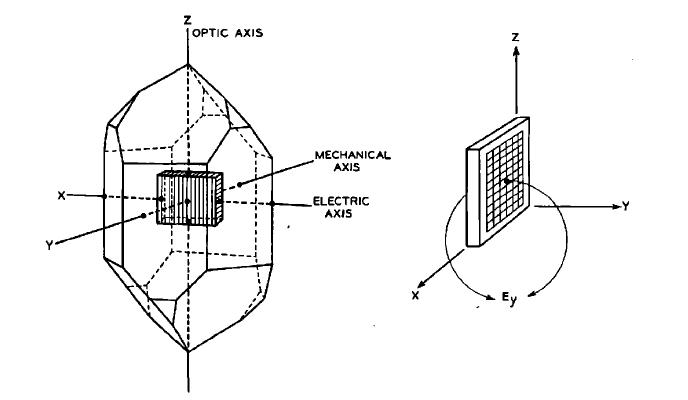
\includegraphics[width=1.0\textwidth]{Chapter-2/fig3_Y_cut_crystal}
	\caption{Representation of how the Y-cut crystal is sectioned from a larger quartz crystal sample. Additionally, the direction of electric field application, for oscillator use, is shown.\cite{211}}
	\label{fig3:Y cut crystal}
\end{figure}





Looking to improve the stability of their their oscillators, researchers at Bell Systems explored the effects of rotating the cut of the crystal by a rotation about the crystallographic x-axis of 31 degrees. This change resulted in drastically improved frequency stability of the resultant oscillator without a proportional loss of piezo-electric activity, as shown in figure 4.


\begin{figure}[hbtp]
	\centering
	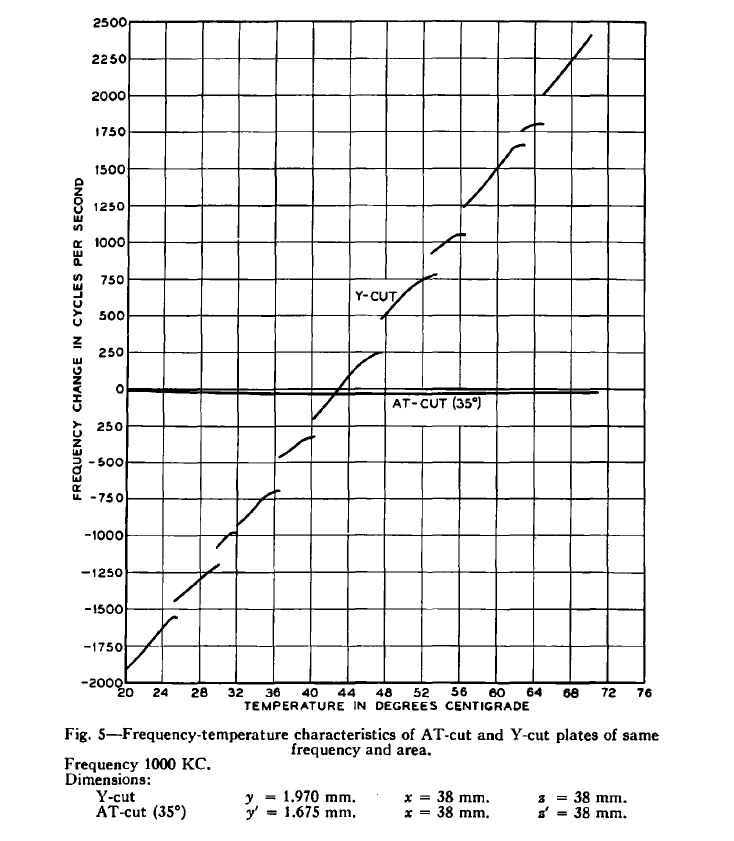
\includegraphics[width=1.0\textwidth]{Chapter-2/fig4_df_vs_T_for_AT_and_Y_cuts}
	\caption{Shift in baseline frequency as a function of temperature for Y-cut and AT-cut crystals, for which temperature stability is improved.\cite{211}}
	\label{fig4:df vs T}
\end{figure}



\subsection{Frequency Shift - Measured}



The crystal oscillators have a stable equilibrium operation mode in both vacuum and aqueous media. In our laboratory tests a frequency drift of less than 1 Hz per hour in aqueous media and performance better than 0.5 Hz per hour in vacuum is typical. For these reasons, the sensitivity to changes in mass at the QCM interface is of great scientific value. While frequency shifts are largely a result of mass-loading, it is critical understand other influences on an observed shift in the QCM frequency during an experiment.



\subsubsection{Mass-loading}

Investigation of rigid-mass-loading on the surface of the QCM was pioneered by M. Sauerbrey, then living in Germany, 1959. Sauerbrey treated adsorbed mass as a small addition to the thickness of the AT-cut (transverse or shear mode) QCM oscillator. \cite{26,27}]

Consider the acoustic, shear-mode oscillation, having speed $\mathit{c_{q}}$ which propagates through the crystal as a product of an applied voltage. The speed of this wave may be decomposed into its wavelength, $\lambda_{q}$ and frequency, $\mathit{f_{q}}$:
	
\begin{equation}
\mathit{c_{q}} = \lambda_{q} \mathit{f_{q}}
\end{equation}
 
Given a crystal fabricated to have a thickness equal to one-half the wavelength of the wavelength above:

\begin{equation}
\mathit{t_{q}} =  \frac{1}{2} \lambda_{q}
\end{equation}

When a film of material is deposited on the surface, the thickness of the oscillator is increased. As can be seen from equations 2.2 and 2.3 above, an increase in oscillator thickness allows an increase in the wavelength, $\lambda_{q}^{'}$ and a decrease in the frequency, $\mathit{f_{q}^{'}}$. The speed of the acoustic wave is assumed to remain constant in the crystal.

\begin{equation}
\mathit{c_{q}} = \lambda_{q}^{'} \mathit{f_{q}^{'}}
\end{equation}

If we take the new film on the surface of the oscillator, having thickness $\mathit{t_{film}}$, and add it to the thickness of the quartz oscillator, $\mathit{t_{q}}$ and recalling that we work from the assumption that the film is rigidly attached to the oscillator's surface, we may right the new thickness of the oscillator $\mathit{t^{'}}$ as:

\begin{equation}
\mathit{t'}= \mathit{t_{film}} + \mathit{t_{q}}
\end{equation}

Bringing in the rigidly-attached film's mass, $\mathit{m_{film}}$, surface area $A$, and with the film's thickness previously defined as $\mathit{t_{film}}$, we may then write the mass density, $\rho_{film}$, of the film as

\begin{equation}
\rho_{film} =  \frac{m_{film}}{A t_{film}}
\end{equation}

Solving equation 2.2 for $\lambda$ and combining it with equation 2.3 produces

\begin{equation}
\mathit{f_{o}} = \frac{c_{q}}{2t_{q}}
\end{equation}

Our interest is in how the frequency changes as a function of the addition of an adsorbed film, so we might differentiate the frequency $f$ in equation 3.6 with respect to the changing thickness of the system, $t'$

\begin{equation}
\frac{\mathrm{d}f_{q} }{\mathrm{d} t_{q}} = \frac{\mathrm{d} }{\mathrm{d}t_{q}}\frac{c_{q}}{2t_{q}}
\end{equation}

Examining equations 2.7 and 2.8 closely for which terms might be cancelled out by operating one on the other, a maneuver appears. Dividing equation 2.7 by equation 2.8 produces

\begin{equation}
\frac{\mathrm{d}f_{q}}{f_{q}} = \frac{-\mathrm{d}t_{q}}{t_{q}}
\end{equation}

Taking a brief detour backwards, re-arrange equation 2.6 to solve for the film's mass, $\mathit{m_{film}}$
\begin{equation}
\mathit{m_{film}} = \rho_{film}A t_{film}
\end{equation}

Our interest is in how a small change of the frequency of the oscillator, a directly measurable quantity, can be utilized to learn the change in mass on the QCM surface in the form of that added film thickness.

\begin{equation}
\Delta \mathit{m_{film}} = \rho_{film}A \Delta t_{film}
\end{equation}

Saurbrey's idea was that if a film were to be considered to be rigidly attached to the surface of the oscillator, then the layer of added material under consideration should be approaching the infintesimal, and so equation 2.11 moves towards that limit to produce


\begin{equation}
d\mathit{m_{film}} = \rho_{film}A dt_{film}
\end{equation}

Equation 2.9, which describes the relative, infinitesimal change in frequency associated the relative, infinitesimal change in the crystal's thickness now seems an appropriate place to substitute in equation 2.12 after it has been solved for change in film thickness, $dt_{film}$

\begin{equation}
\frac{\mathrm{d}f_{q}}{f_{q}} = \frac{-\mathrm{d}m_{film}}{t_{q}\rho_{film}A}
\end{equation}

Recall that we are principally interested, with this treatment, in loading the QCM with a mass such that $dm_{film} << m_{q}$. Defining the speed of the sheer oscillation as $v_{q} = \frac{f_{q}}{\lambda_{q}}$, the widely-reknowned Saurbrey Equation for one-sided film-growth is written
\begin{equation}
\Delta f = \frac{-\Delta m_{film}f_{q}^{2}}{A\rho_{film}v_{q}}
\end{equation}

The above relationship may be used to convert a measured shift in the resonant frequency of the QCM to a value for mass added to the interface of the QCM if the adhered film:

\begin{enumerate}
	\item covers the portion of the QCM which is in motion uniformly
	\item is non-dissipative (no slip OR slip with zero friction?)
	\item has a mass which is much smaller than the mass of the oscillator as a whole
	\item is rigidly attached to the surface
\end{enumerate}

The Saurbrey equation, and his reasoning, are a special case for the interaction of an adsorbed film on the surface of an oscillating quartz crystal microbalance. Despite several decades of use since his work, and more general approaches being developed, the Saurbrey equation remains a gold standard for nanotribology. Mass-loading is responsibile for the greatest portion of frequency shifts observed for the work reported in this thesis.









\subsection{Energy Dissipation at the QCM Interface}

\subsubsection{Amplitude - Measured}

Amplitude of oscillation, in volts, is the other quantity measured from a QCM in operation.  Generally speaking, as the amount of energy lost at the interface between the QCM surface and its counter-face increases, the amplitude will decrease. This is not a complete picture as the QCM-oscillator-system may also lose energy internally.


\subsubsection{Quality Factor}

The quality factor, $Q$, describes the degree of damping in an oscillating system. The QCM system is an electrical circuit driving a physical oscillator, both of which feedback into the other. Provided that the electronics are well-insulated from disturbance, the a shift in Q, for the QCM system, indicates and increase or decrease in energy dissipation at the interface. A useful,  definition for $Q$ is given as follows in equation 2.15:

\begin{equation}
Q = 2* \Pi* \frac{Energy Added per Cycle}{Energy Lost per Cycle}
\end{equation}

Electrical energy is added to the system by driving circuitry while dissipation of energy occurs either through inter-facial or internal mechanisms. Inversely proportional to the quality factor is then readily defined as the dissipation factor, $D \alpha Q^{-1}$

\subsection{Slippage at the QCM Interface}

Slippage, or phase delay, between materials and the QCM surface itself results in dissipation of energy. The effect of a film moving out-of-phase with the QCM, ie slipping, has been calculated by Bruschi and Mistura. (L Bruschi and G. Mistura, Phys Rev B 63, 235411 2011).

This slippage at the interface adds a component to the impedance of the system. This is critical for a full treatment of few-molecule adsorbtion to the QCM in vacuum. Additionally, it provides insight into the mechanism by which the QCM in liquid loses energy with each cycle. This additonal impedance is defined as $\frac{1}{\eta_{2}}$.

\subsection{The Behavior of the QCM, in Vacuum, in the Presence of Gaseous Species - Adsorption Isotherms}



\subsection{The Behavior of the QCM in Liquid Environments}

\subsubsection{Temperature}

Use of AT-cut quartz crystals

\subsubsection{Pressure}

\begin{figure}[hbtp]
	\centering
	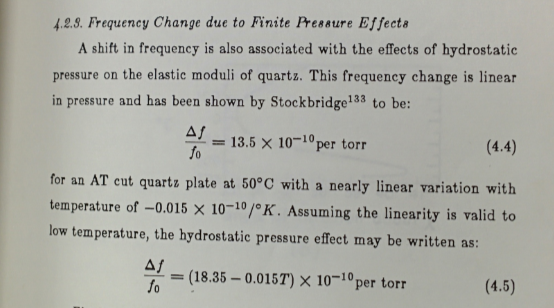
\includegraphics[width=1.0\textwidth]{Chapter-2/fig3_krim_thesis_QCM_pressure_effect}
	\caption{THIS IS A PLACEHOLDER - needs to be swapped for specifics refs to Krim Thesis (1984) and Stockbrige, Ref 133 from that thesis}
	\label{fig5:QCM_pressure}
\end{figure}



\subsubsection{Stress -and changes in pressure?-}

\section{LabVIEW Recording Software for QCM Experiments}


\section{The Atomic Force Microscope}

Observations of surface roughness for materials, before and after their exposure to tribological processes, provides information regarding etching, polishing, or other wear behaviors. The AFM was the principle tool used in this work to characterize material surfaces for these purposes. The principles of operation of the AFM apparatus generally, as well as pertinent speficics of the platform used to take the measurements described in this work, are as follows.



\section{Scanning Electron Microscope}




\section{Vacuum Systems}









\section{Equipment for Liquid-immersed QCM Measurements}



\subsection{Stanford Research Systems Flow Cell}



\subsubsection{Flow Cell Electronics}




\section{Macro-scale Friction Measurements}



\subsection{Background and Conventions for Macro-scale Tribology}

Testing for wear, friction, and lubrication between macro-scale contacts is of obvious importance for nearly any industrial or commercial enterprise which uses stationary machinery or transportation equipment. In the research setting, a macro-scale tribometer is useful as a means of testing novel lubricants or additives. The observations from such macro-scale tests, which are often cheaper, easier, and faster to conduct than many fine or even atomic scale measurements, can contribute to a tighter feedback loop in tribological studies. Critically, employment of a macroscale tribometer allows for correlation between lubrication and wear in practical settings with the behavior of nanoparticles at the interface as observed with other research implements.


\subsection{PCS Instruments MTM-2 Macro-scale Tribometer}



\section{Dynamic Light Scattering and Electrophoresis Measurements for Nanometer Size Particle Characterization}





\subsubsection{Principles of Dynamic Light Scattering}



\subsubsection{Principles of Electrophoresis}

For any set of nanoparticles in aqueous solution, it is necessary that they exhibit a mutual electro-static repulsion lest they agglomerate with one another, changing physical, optical, and other properties of critical interest. The mechanism by which aqueously suspended particles maintain their distance is electro-static repulsion(CITATION NEEDED). Typically characterized by a zeta potential, $\zeta$, measured in millivolts, the degree of repulsion is determined through use of an electrophoresis measurement (CITATION NEEDED).

By applying an electric field across a sufficiently dilute sample, particles within the sample will begin to move parallel to the direction of the field. The speed at which the particles move, on average, is a function of the field strength as well as the net charge, $Q$, on the constituent particles. The force experienced by each particle may be written as follows.

\begin{equation}
\mathit{f} = E \times Q
\end{equation}



The velocity is determined by means of a doppler-shift in a LASER signal directed into the liquid sample.

\subsubsection{Malvern ZetaSizer Specifics}








\addcontentsline{toc}{section}{{Chapter 2 References}}